\section{Continuous Integration}
En Continous integration server er  en server der kan teste et projekts software samlet.
Med samlet, menes der at et project repository, som flere programmører \textit{pusher} til, automatisk kan kompilere, integrere og køre softwaren og de skrevne tests. Softwaren bliver altså bygget sammen med den resterende software der allerede findes på build serveren.

\begin{figure}[H]
\centering
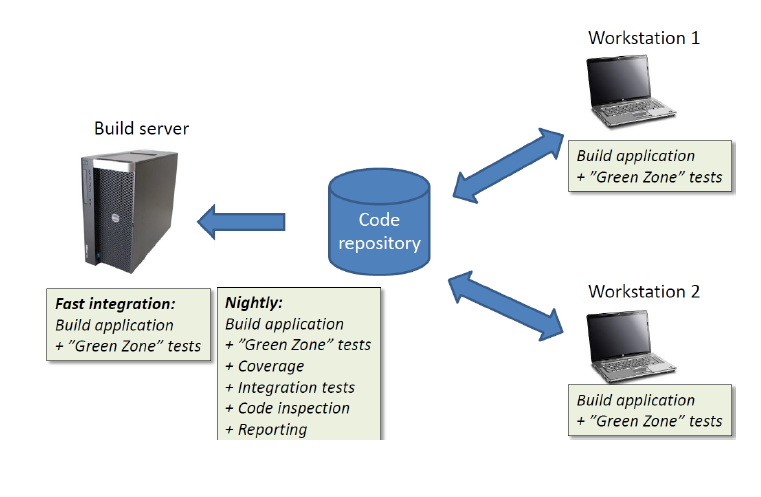
\includegraphics[width=0.7\linewidth]{figs/ciArch.PNG}
\caption{Modellen for Continous Integration i et projekt}
\label{fig:ciArch}
\end{figure}

\subsection{CI funktionalitet}
På figur~\ref{} ses trigger skevensen for et automatisk \textit{\textbf{build}} og \textit{\textbf{run}}.

\begin{figure}[H]
\centering
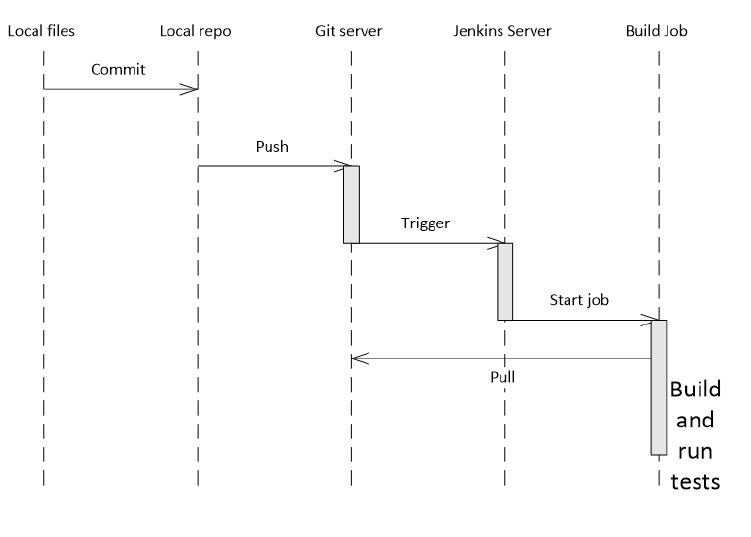
\includegraphics[width=0.7\linewidth]{figs/ciTriggerSeq.PNG}
\caption{Trigger sekvens for Continous Integration med Git repository.}
\label{fig:ciTriggerSeq}
\end{figure}

Fordelene ved Continous Integration er:

\begin{itemize}
	\item Hele projektet testes samlet.
	\item Test sker uden for miljøet - Ved store projekter spares tid.
	\item Der pushes deployable builds \todo{er det et krav at man kun pusher deployable builds i jenkins?}
	\item Der kan pushes ofte, så der findes fejl før der skrives meget kode.
	\item Code metrics/quality er altid opdateret (hvis CI systemet understøtter det).
\end{itemize}

\subsection{CI Systemer}
I SWT arbejdes der med Jenkins serveren. Udover at bygge et software projekt, kører den også tilhørende tests, hvorefter den kan sende en mail om resultatet.
Jenkins mantra: build, test, result, mail. \todo{Er det en ting det her?}

Derudover er der en stor del funktionalitet i Jenkins. Herunder Code Coverage og Metrics.

\todo{lav eksempel med ATM opgaven}

\todo{skriv om Travis og evt. forskelle mellem Jenkins og Travis}